\documentclass[landscape,footrule]{foils}
\usepackage[lecture-serie]{foiltex-extra}
\usepackage{crysymb}
\usepackage{graphics}
\usepackage[dvipsnames]{xcolor}
%\usepackage[utf8]{inputenc}
%\usepackage{fontspec}
\usepackage[pdftex]{graphicx} 




\newcommand{\lecture}{ A practical guide to information extraction from medical texts}
\newcommand{\lserie}{3rd MLFPM Summer School}
\newcommand{\ldate}{21 September, 2021}
\newcommand{\lauthor}{Sven Laur}
\newcommand{\linst}{University of Tartu}
\graphicspath{{./illustrations/}}
\MyLogo{\lserie,\ Information extraction from medical texts, \ldate}


\newcommand{\leqm}{\ \leq_m}


\newcommand{\bigvskip}{\vskip 2em}
\newcommand{\lastline}{\vspace*{-2ex}}
\newcommand{\spreadappart}{\vspace*{\fill}}

\DeclareMathOperator{\supp}{supp}
\DeclareMathOperator{\conf}{conf}
\DeclareMathOperator{\precision}{precision}
\DeclareMathOperator{\recall}{recall}


\begin{document}
\titlefoil

\foilhead[-1cm]{Why information extraction is needed}

Electronic health records are mostly unstructured:
\begin{diamonds}
 \item patient complaints (\textcolor{blue}{adverse drug reactions})
 \item disease descriptions are textual (\textcolor{blue}{deep phenotyping})
 \item biopsies have textual descriptions (\textcolor{blue}{cancer studies})
 \item descriptions of X-ray scans are textual (\textcolor{blue}{label assignment})\vspace*{3ex}
\end{diamonds}\vspace{1cm}

Information extraction allows us: 
\begin{diamonds}
\item to fill gaps in the structured data (\textcolor{blue}{allergies})
\item to describe environment factors (\textcolor{blue}{lifestyle and family history})
\item to refine diagnosis description (\textcolor{blue}{infraction subtypes}) 
\item to refined treatment outcomes (\textcolor{blue}{stroke complications}) 
\end{diamonds}


\foilhead[-1cm]{Example. Measurement extraction}

Extract dated lab measurements from a patient health record.\vspace*{1cm}


\centerline{\includegraphics[width=18cm, trim= 0cm -0.25cm 0cm 0cm, clip]{measurement-extraction-task}}


\foilhead[-1cm]{NLP tasks in medical domain}

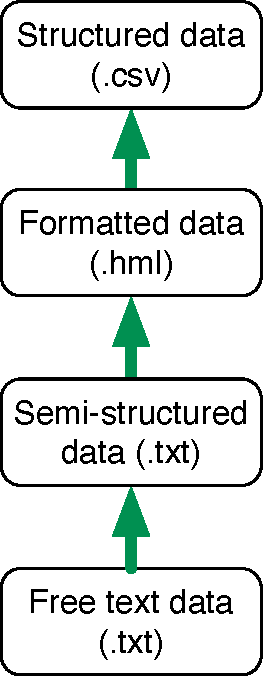
\includegraphics[scale=1.0, trim= 0cm -0.25cm 0cm 0cm, clip]{nlp-tasks}\hspace*{0.5cm}
\begin{minipage}[b]{16cm}
\begin{triangles}
\item Cleaning individual values (\textcolor{blue}{1, 3 $\leadsto$ 1.3})
\item Standardisation of terms (\textcolor{blue}{penicillin $\leadsto$ J01C})
\item Harmonisation and conflict resolution
\end{triangles}\vspace*{3ex}
\begin{triangles}
\item Extraction of individual data fields
\item Unification of different data formats
\end{triangles}\vspace*{3ex}
\begin{triangles}
\item Format discovery
\item Robust parsing 
\item Text segmentation
\end{triangles}
\vspace*{3ex}
\begin{triangles}
\item Text segmentation
\item Relevance ranking
\item Fact extraction
\end{triangles}
\end{minipage}




\foilhead[-1cm]{How to carry out information extraction}

\illustration[scale=0.9]{ie-choices}

\foilhead[-1cm]{Typical steps for a fact extraction task}

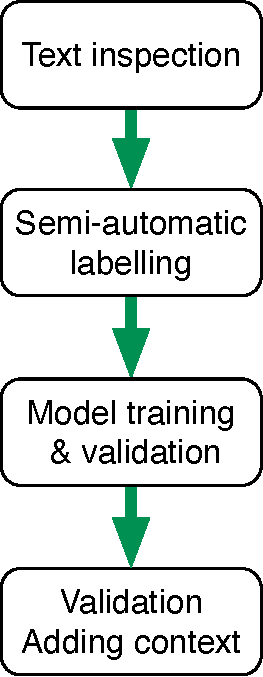
\includegraphics[scale=1.0, trim= 0cm -0.25cm 0cm 0cm, clip]{steps-in-fact-extraction-task}\hspace*{0.5cm}
\begin{minipage}[b]{16cm}
\includegraphics[scale=0.7, trim= 0cm 0.1cm 1cm 0cm, clip]{text-inspection}
\vspace*{-2ex}
\begin{triangles}
\item Term lists and regular expressions 
\item Text segmentation and focus regions
\item Dataset enrichment.  Manual corrections 
\end{triangles}\vspace*{3ex}
\begin{triangles}
\item Detection and extraction tasks
\item Text prioritisation task
\end{triangles}\vspace*{5ex}
\begin{triangles}
\item Plausibility (\textcolor{blue}{Weight: 1.63 kg})
\item Context (\textcolor{blue}{Weight: 3.4 kg 30 year female})
\vspace*{2ex}
\end{triangles}
\end{minipage}




\foilhead[-1cm]{Abstraction levels in text mining}

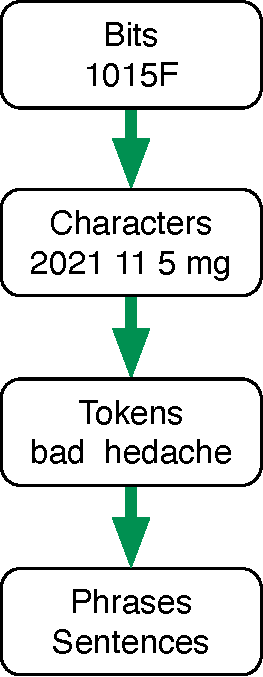
\includegraphics[scale=1.0, trim= 0cm -0.25cm 0cm 0cm, clip]{abstraction-levels-in-text-mining}\hspace*{0.5cm}
\begin{minipage}[b]{17cm}
\begin{triangles}
\item Charset detection (\textcolor{blue}{utf-8, Latin-1, Windows-1257})
\item Recovery from encoding errors (\textcolor{blue}{\hspace*{-0.2ex}\raisebox{-0.8ex}{
\includegraphics[scale=1]{jyrioo-1.pdf}} $\leadsto$ j\"uri\"o\"o}) 
\end{triangles}\vspace*{3ex}
Tokenisation
\begin{triangles}
\item number and abbrevation detection (\textcolor{blue}{weight 1, 3 kg})
\item word normalisation (\textcolor{blue}{hedache$\leadsto$headache, ug$\leadsto$ $\mu$g})
\end{triangles}\vspace*{3ex}

Token-level annotations 

\begin{triangles}
\item morphological analysis (\textcolor{blue}{cramped $\leadsto$ verb, past tense})
\item term ontologies (\textcolor{blue}{penicillin $\leadsto$ J01C, liver $\leadsto$ abdomen})
\end{triangles}
\vspace*{3ex}
Phrase level analysis
\begin{triangles}
\item text segmentation and relevance ranking (\textcolor{blue}{focus})
\item fact extraction and text quantification (\textcolor{blue}{prediction})
\end{triangles}
\end{minipage}

\foilhead[-1cm]{Commonly used methods}
\enlargethispage{1cm}

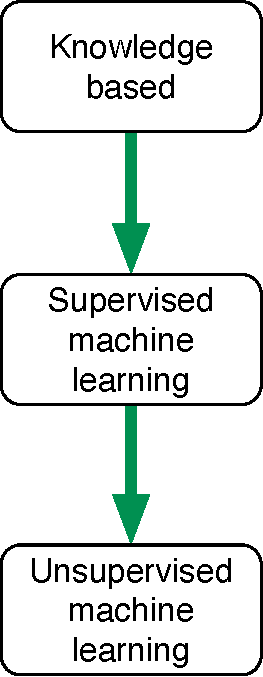
\includegraphics[scale=1.0, trim=0cm -1.375cm 0cm 0cm, clip]{methods-hierarchy}
\hspace*{0.5cm}
\begin{minipage}[b]{12cm}
Rule-based methods 
\begin{triangles}
\item term lists 
\item regular expressions \& rewriters
\item phrase grammars    
\end{triangles}\vspace*{4ex}
Supervised machine learning
\begin{triangles}
\item text segmentation
\item text classification 
\item keyword assignment
\end{triangles}\vspace*{3ex}

Unsupervised machine learning 
\begin{triangles}
\item word embeddings (\textcolor{blue}{\textsc{Word2vec}}) 
\item transformers (\textcolor{blue}{\textsc{Bert} \& \textsc{Gpt-3}}) 
\item similarity scoring (\textcolor{blue}{\textsc{Wmd}})
\end{triangles} \vspace*{2ex}
\end{minipage}
\hspace*{0.5cm}
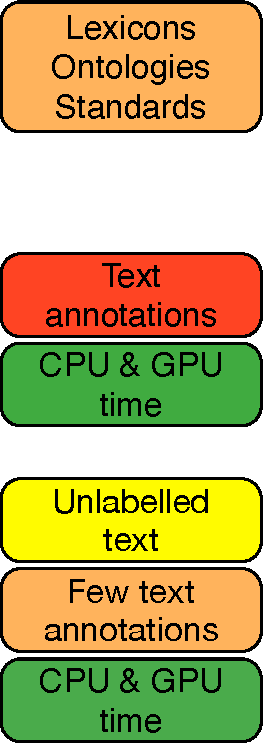
\includegraphics[scale=1.0, trim=0cm -0.5cm 0cm 0cm, clip]{resource-hierarchy}

\middlefoil{Rule-based methods}

\foilhead[-1cm]{Standards as the source of term lists}

\begin{minipage}[b]{12cm}
Disease names 
\begin{diamonds}
\item \textsc{Icd-10}, \textsc{Snomed-CT}
\end{diamonds}\vspace*{4ex}

Lab measurements
\begin{diamonds}
\item \textsc{Loinc}, \textsc{Snomed-CT}
\end{diamonds}\vspace*{4ex}

Drug names and adverse reactions
\begin{diamonds}
\item \textsc{Atc}, \textsc{Snomed-CT}
\item drug package leaflets
\end{diamonds}\vspace*{4ex}

Anatomy
\begin{diamonds}
\item  \textsc{Aeo}, \textsc{Caro}, \textsc{Snomed-CT}
\item medical dictionaries
\end{diamonds}
\vspace*{3ex}
\end{minipage}
\hspace*{0.5cm}
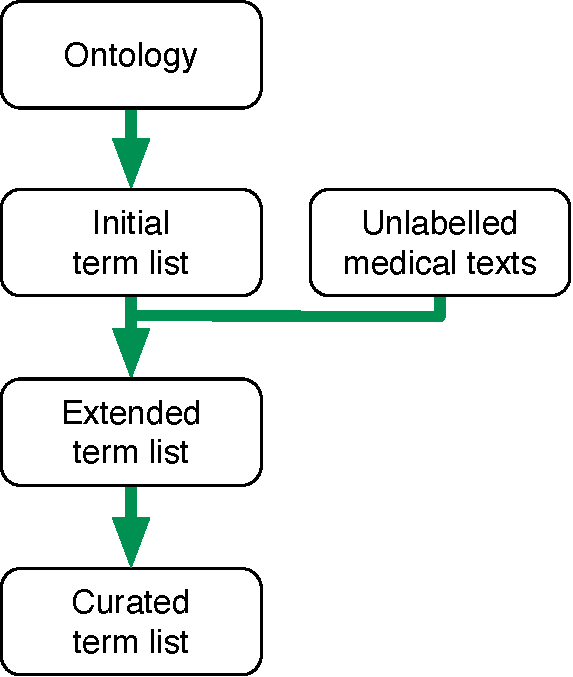
\includegraphics[scale=1.0, trim=0cm -0.25cm 0cm 0cm, clip]{term-extraction}


\foilhead[-1cm]{Tokenisation with regular expressions}

\renewcommand{\verb}{\collectverb{\color{red}}}
Regular expression is a way to specify tokens with fixed structure:
\begin{triangles}
\item dates (\textcolor{blue}{\texttt{[0-9]\^{}2.[0-9]\^{}2.[0-9]\^{}4}}) 
\item number formats (\textcolor{blue}{\texttt{-?[0-9]\^{}+.[0-9]\^{}+}}) 
\item special symbols, headers
\end{triangles} \vspace*{3ex}

Do \textbf{not} use regular expression for predictable variations in term lists.
\begin{triangles}
\item handling long term lists is much more efficient.  
\item you might get \textcolor{blue}{\texttt{a|ab|abc}} vs \textcolor{blue}{\texttt{abc|ab|a}} problems.
\end{triangles} \vspace*{3ex}

Software development practices:
\begin{triangles}
\item Write test cases for each surprise. 
\item Maintain common library of regular expressions.    
\end{triangles}   


\foilhead[-1cm]{What is a phrase grammar}

A phrase grammar is a list of rules that combines tokens into phrases:
\begin{align*}
\textsc{Number}\; \textsc{Unit} &\leadsto \textsc{QNumber}\\
\textsc{Date}\;\textsc{Analyte}\; \textsc{QNumber} &\leadsto \textsc{Measurement}\\
\textsc{Analyte}\; \textsc{QNumber} &\leadsto \textsc{Measurement}\\
\textsc{Date}\; \textsc{Analyte}\; \textsc{Number} &\leadsto \textsc{Measurement}\\
\textsc{Analyte}\; \textsc{Number} &\leadsto \textsc{Measurement}
\end{align*} 

\begin{triangles}
\item There can be several phrase symbols of interest.
\item If many rules apply the one with highest priority is applied. 
\item Rules can specify how to compute extra attributes for derived symbols. 
\item All phrase grammars classes are finite in practice. 
\end{triangles}



\foilhead[-1cm]{Illustrative example}

Canonical phrase \vspace*{2ex}

\centerline{
\colorbox{Orchid!80}{\texttt{21.05.2021}}
\colorbox{OliveGreen!80}{\texttt{Cholesterol}}
\colorbox{Orange!80}{\texttt{100.2}}
\colorbox{Red!80}{\texttt{m\smash{g/}dL}}}
\centerline{\rotatebox{-90}{$\leadsto$}}\vspace*{1.5ex}
\centerline{$\textsc{Measurement}(date=2021/05/21, analyte = Cholesterol, \ldots)$}
\vspace*{4ex}

Incomplete phrases we must match

\begin{triangles}
\item 
\colorbox{OliveGreen!80}{\texttt{Cholesterol}}
\colorbox{Orange!80}{\texttt{100.2}}
\colorbox{Red!80}{\texttt{m\smash{g/}dL}}
\item 
\colorbox{Orchid!80}{\texttt{21.05.2021}}
\colorbox{OliveGreen!80}{\texttt{Cholesterol}}
\colorbox{Orange!80}{\texttt{100.2}}
\item 
\colorbox{OliveGreen!80}{\texttt{Cholesterol}}
\colorbox{Orange!80}{\texttt{100.2}}
\end{triangles}


\foilhead[-1cm]{Advanced tricks}

Incomplete phrases reveal missing knowledge
\begin{triangles}
\item 
\colorbox{Orchid!80}{\texttt{21.05.2021}}
\colorbox{Gray!80}{\texttt{HDL}}
\colorbox{Orange!80}{\texttt{20.3}}
\colorbox{Red!80}{\texttt{m\smash{g/}dL}}
\item 
\colorbox{Orchid!80}{\texttt{21.05.2021}}
\colorbox{OliveGreen!80}{\texttt{Cholesterol}}
\colorbox{Orange!80}{\texttt{406}}
\colorbox{Gray!80}{\texttt{m\smash{g/}L}}
\vspace*{3ex}

\end{triangles}

Additional checks
\begin{triangles}
\item 
\texttt{Last measurement of}
\colorbox{OliveGreen!80}{\texttt{Cholesterol}}
\colorbox{Orange!80}{\texttt{2005}}

\end{triangles}
\vspace*{3ex}

Tokenisation is ambiguous in practice
\begin{triangles}
\item 
\colorbox{OliveGreen!80}{\texttt{Cholesterol}}
\colorbox{Orchid!80}{\texttt{21.05 2021}}
\colorbox{Orange!80}{\texttt{40.6}}\texttt{; }
\colorbox{OliveGreen!80}{\texttt{HDL}}
\item 
\colorbox{OliveGreen!80}{\texttt{Cholesterol}}
\colorbox{Orange!80}{\texttt{21.05}}
\texttt{2021\hspace*{1em}40.6}
\texttt{; }
\colorbox{OliveGreen!80}{\texttt{HDL}}
\end{triangles}


\foilhead[-1cm]{Conclusion}

Advantages of rule-based methods:
\begin{triangles}
\item Easy to achieve decent progress.
\item Do not need extensive manual annotations.
\item A good baseline for segmentation tasks.   
\end{triangles}
\vspace*{2cm}

Disadvantages of rule-based methods:
\begin{triangles}
\item Manual derivation of rules is hard.
\item Curation of background information is hard.
\item Progressively harder to improve the performance. 
\end{triangles}
\vspace*{3ex}

\middlefoil{Supervised machine learning}

\foilhead[-1cm]{Support Vector Machines}

Linear classifier is an automatic way to derive implicit rules from examples
\begin{align*}
f(x)=1\times \colorbox{OliveGreen!80}{\texttt{Cholesterol}}(x) + 1\times \colorbox{OliveGreen!80}{\texttt{HDL}}(x) + 1\times\colorbox{OliveGreen!80}{\texttt{LDL}}(x) - 2 
\end{align*}  
\centerline{$\Updownarrow$}
\begin{align*}
\colorbox{OliveGreen!80}{\texttt{Cholesterol}}(x) \wedge \colorbox{OliveGreen!80}{\texttt{HDL}}(x)&=\textsc{True}\\
\colorbox{OliveGreen!80}{\texttt{HDL}}(x) \wedge \colorbox{OliveGreen!80}{\texttt{LDL}}(x)&=\textsc{True}\\
\colorbox{OliveGreen!80}{\texttt{Cholesterol}}(x) \wedge \colorbox{OliveGreen!80}{\texttt{LDL}}(x)&=\textsc{True}
\end{align*}

Support Vector Machine is \emph{statistically stable way} to do linear classification.

\begin{triangles}
\item Feature maps and kernels allow to do nonlinear combination of features.
\end{triangles}


\foilhead[0cm]{Manual feature engineering}

\centerline{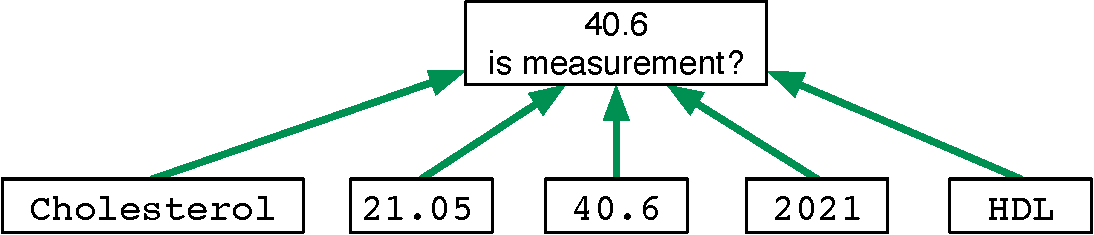
\includegraphics[scale=1.0, trim= 0cm 0.0cm -3cm 0cm, clip]{prediction-window}}

The quality of predictions mostly depends on available features:
\begin{triangles}
\item term lists
\item phrase lists
\item morphological features
\item size of the window
\end{triangles}  

\foilhead[-1cm]{Output smoothing with CRF}
\enlargethispage{3cm}

\begin{triangles}
\item The predictions of SVM are independent for each position.\vspace*{1ex}

\colorbox{OliveGreen!80}{\texttt{21.05}} \texttt{2021}
\colorbox{OliveGreen!80}{\texttt{Cholesterol}}
\colorbox{OliveGreen!80}{\texttt{40.6}}
\colorbox{White}{\texttt{;}}
\colorbox{Orange!80}{\texttt{HDL}}
\colorbox{OliveGreen!80}{\texttt{16.3}}
\colorbox{Orange!80}{\texttt{m\smash{g/d}L}}
\vspace*{2ex}

\item Consistency requirements can be modelled with Markov random fields. \vspace*{1ex}

\colorbox{OliveGreen!80}{\phantom{\texttt{21.05}}} \phantom{\texttt{2021}}
\colorbox{OliveGreen!80}{\phantom{\texttt{Cholesterol}}}
\colorbox{OliveGreen!80}{\phantom{\texttt{40.6}}}
\colorbox{White}{\phantom{\texttt{;}}}
\colorbox{Orange!80}{\phantom{\texttt{HDL}}}
\colorbox{OliveGreen!80}{\phantom{\texttt{16.3}}}
\colorbox{Orange!80}{\phantom{\texttt{m\smash{g/d}L}}}
\vspace*{-1ex}

\centerline{\rotatebox{-90}{$\leadsto$}}\vspace*{0ex}
\centerline{very unlikely}
\vspace*{2ex}

\item Conditional Random Fields smooths independent predictions.\vspace*{1ex} 

\colorbox{OliveGreen!80}{\texttt{21.05}} 
\colorbox{White}{\texttt{2021}}
\colorbox{OliveGreen!80}{\texttt{Cholesterol}}
\colorbox{OliveGreen!80}{\texttt{40.6}}
\colorbox{White}{\texttt{;}}
\colorbox{Orange!80}{\texttt{HDL}}
\colorbox{OliveGreen!80}{\texttt{16.3}}
\colorbox{Orange!80}{\texttt{m\smash{g/d}L}}
\vspace*{-1ex}

\centerline{\rotatebox{-90}{$\leadsto$}}\vspace*{0.5ex}

\colorbox{OliveGreen!80}{\texttt{21.05}} 
\colorbox{OliveGreen!80}{\texttt{2021}}
\colorbox{OliveGreen!80}{\texttt{Cholesterol}}
\colorbox{OliveGreen!80}{\texttt{40.6}}
\colorbox{White}{\texttt{;}}
\colorbox{Orange!80}{\texttt{HDL}}
\colorbox{Orange!80}{\texttt{16.3}}
\colorbox{Orange!80}{\texttt{m\smash{g/d}L}}
\vspace*{2ex}

\end{triangles} 

\foilhead[-1cm]{Word embeddings}

Word embedding defines 100-1000 informative features for each word.
\begin{triangles}
\item Features are defined automatically. 
\item Masked language modelling is used for training.
\item Each word gets a fixed representation vector.
\item Cosine similarity between embeddings indicates semantical closeness.
\end{triangles}
\vspace*{2cm}

By running SVM on top of embeddings: 
\begin{triangles}
\item We do not need to hand-crafting word-based features. 
\item We still have to think about the window size. 
\item We have to fix the amount of unknown words.
\item We ignore that words can have multiple meanings.
\end{triangles}

\foilhead[-1cm]{Context sensitive word embeddings}

Neural networks define informative features for each occurrence of the word.

\begin{triangles}
\item Features are defined automatically. 
\item Masked language modelling is used for training.
\item There is no observation window -- information can flow.  
\item Different meanings of the words get different representations.
\item Sentences or paragraphs get also representations.
\end{triangles}
\vspace*{2.5cm}

By running a neural network on top of context-sensitive embeddings: 
\begin{triangles}
\item We can adjust the baseline representation for current task. 
\item We still cannot capture dark background knowledge. 
\end{triangles}


\middlefoil{Iterative improvement}


\foilhead[-1cm]{Three main sources of improvement}

Improve the quality of term lists and ontologies.
\begin{triangles}
\item Use version control smartly to communicate changes 
\end{triangles}
\vspace*{1.5cm}

Extraction quality does not increase if you do not measure it!
\begin{triangles}
\item Create dedicated test sets for each isolated problem.
\end{triangles}
\vspace*{1.5cm}


Use external consistency checks to discover errors. 
\begin{triangles}
\item Any test that works unlabelled data is good.
\item Automatic checks for statistical anomalies.
\end{triangles}

\foilhead[-1cm]{Diminishing returns}

\centerline{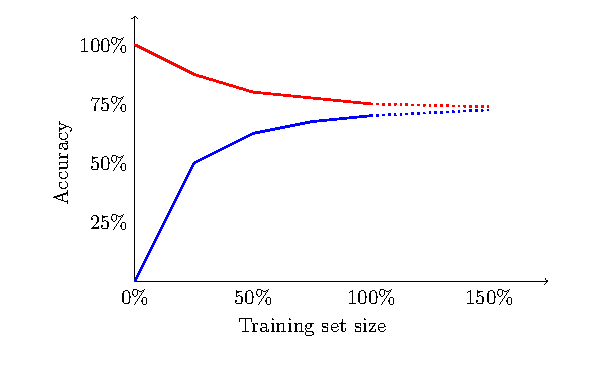
\includegraphics[scale=1.5, trim= 0cm 0.0cm 0cm 0cm, clip]{performance-vs-data}}

Most machine learning problems are not solvable by collection more samples.

\begin{triangles}
\item By reducing training set size it one can estimate potential gains.
\end{triangles} 



\foilhead[-1cm]{Pitfalls of absolute performance measures}

\centerline{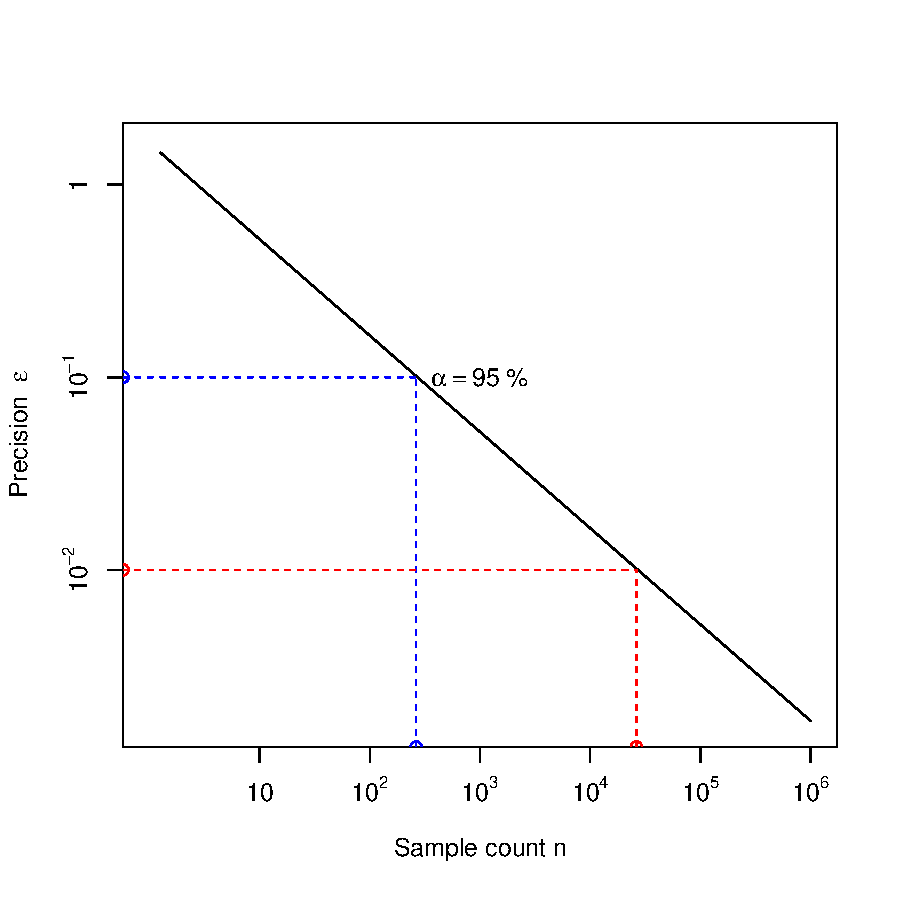
\includegraphics[scale=0.6, trim= 0cm 0.5cm 0cm 1cm, clip]{sampling-bounds}}

Test error estimates are not very precise: 
\begin{triangles}
\item To increase precision 10 time you need 100 times more data.
\item You can estimate test error with precision $1\%$ not more.
\item You cannot reliably detect progress on a reasonable test set.
\end{triangles}


\foilhead[-1cm]{Relative performance}

Unlabelled data can be used for more precise performance estimates:

\begin{triangles}
\item Fix a good base line model.
\item Evaluate both models on unlabelled data.
\item Choose uniformly at random 100 - 1000 prediction differences.
\item Establish the ground truth for these differences.
\item Compute improvement ratio for differences.
\item Compute relative frequency of difference.
\item Their multiple is the relative performance gain.   
\end{triangles}  


\end{document}

